\documentclass{article}

\usepackage[mast]{dennis}

\title{Diagnostic + Quiz 1 Discussion!}
\author{Dennis Chen}
\date{Meet 1}

\begin{document}
\maketitle

\part{Diagnostic Discussion}

\section*{Comments}

% too much geo (in proof)

\pagebreak\section{Question 1}

How many integer values of $1\leq x\leq 100$ makes $x^2+8x+5$ divisible by $10?$

\subsection{Solution}

Complete the square.

$(x+4)^2\equiv 1\pmod{10},$ so there's clearly two solutions mod $10.$

My way (probably worse):

$x^2+8x+5\equiv (x+3)(x+5)\pmod{10}$

\pagebreak\section{Question 2 (QIDb602's Memorial Mock AMC 10)}

In the following diagram, $m\angle BAC=m\angle BFC=40^{\circ}$, $m\angle ABF=80^{\circ}$, and $m\angle FEB=2m\angle DBE=2m\angle FBE$. What is $m\angle ADB$?

    \begin{center}
        \begin{asy}
        import olympiad;
        size(4cm);
    draw((0,0)--(-14,0)--(2,8)--(0,0)--(-9,2.5)--(-5.5,0)--(-6,4)--cycle);
    draw((-5.5,0)--(2,8));
    label("A", (2,8), NE);
    label("B", (0,0), SE);
    label("C", (-5.5,0), S);
    label("D", (-14,0), SW);
    label("E", (-9,2.5), NNW);
    label("F", (-6,4), NNW);
        \end{asy}
    \end{center}

\subsection{Solution}

The most blatant thing is $\angle BAC=\angle BFC=40,$ so $BAFC$ is cyclic.

So $\angle ABF=\angle ACF=80.$

Also do some angle chasing and realize $DEB$ is isosceles.

So in the end the answer is $\angle ADB=\angle EDB=12.$

\pagebreak\section{Question 3}

Consider parallelogram $ABCD$ with $AB=7,$ $BC=6.$ Let the angle bisector of $\angle DAB$ intersect $BC$ at $X$ and $CD$ at $Y.$ Let the line through $X$ parallel to $BD$ intersect $AD$ at $Q.$ If $QY=6,$ find $\cos\angle DAB.$

\subsection{Solution}

\begin{itemize}
	\item Notice $\triangle ABX$ is isosceles
	
	\item Similarly, $\triangle ADY$ is isosceles
	
	\item Also, $XQDB$ is a parallelogram
\end{itemize}

This gives us $DY=6$ and $QD=XB=AB=7.$ Since $\angle QDY=\angle DAB,$ just finding $\cos \angle QDY$ is sufficient.

\begin{asy}
size(4cm);
dot((0,0));
label("$A$",(0,0),SW);
dot((7,0));
label("$B$",(7,0),SW);
dot((7/2,sqrt(95)/2));
label("$D$",(7/2,sqrt(95)/2),NW);
dot((21/2,sqrt(95)/2));
label("$C$",(21/2,sqrt(95)/2),SE);
dot((19/2,sqrt(95)/2));
label("$Y$",(19/2,sqrt(95)/2),N);
dot((133/12,7sqrt(95)/12));
label("$X$",(133/12,7sqrt(95)/12),NE);
dot((91/12,13sqrt(95)/12));
label("$Q$",(91/12,13sqrt(95)/12), NW);

draw((0,0)--(133/12,7sqrt(95)/12));
draw((91/12,13sqrt(95)/12)--(133/12,7sqrt(95)/12));
draw((0,0)--(91/12,13sqrt(95)/12));
draw((0,0)--(7,0)--(133/12,7sqrt(95)/12));
draw((21/2,sqrt(95)/2)--(7/2,sqrt(95)/2));
\end{asy}

\subsection{0 brain cells}
Literally just use slanted coordinate axes and win. Notice the angle bisector has equation $y=x,$ everything else is trivial from there.

\pagebreak\section{Question 4}

Consider unit circle $O$ with diameter $AB.$ Let $T$ be on the circle such that $TA<TB.$ Let the tangent line through $T$ intersect $AB$ at $X$ and intersect the tangent line through $B$ at $Y.$ Let $M$ be the midpoint of $YB,$ and let $XM$ intersect circle $O$ at $P$ and $Q.$ If $XP=MQ,$ find $AT.$

\subsection{Solution}

Let $O$ be the center of the circle. Notice that this implies that $OM=OX.$ We claim that if $BM=x,$ then $XT=x$ as well.
    
Do some PoP stuff and notice $XT=MB.$
    
    \begin{asy}
    size(6cm);
label("$B$", (0,0), SW);
label("$O$", (1,0), S);
label("$A$", (2,0), SE);
label("$X$", (2.5,0), SE);
label("$M$", (0,sqrt(5)/2), W);
label("$Y$", (0,sqrt(5)), NW);
label("$T$", (5/3,sqrt(5)/3), NE);
dot((0,0));
dot((1,0));
dot((2,0));
dot((2.5,0));
dot((0,sqrt(5)/2));
dot((5/3,sqrt(5)/3));
dot((0,sqrt(5)));
draw((0,0)--(2.5,0)--(0,sqrt(5))--cycle);
draw(circle((1,0),1));
    \end{asy}

With this information, we can actually find the scale of the triangle.

Say $XT=MB=x,$ then $YB=2x$ and $YT=2x$, so $YX=3x.$ And $XB=\sqrt{5}x.$

% Also, by the Pythagorean Theorem, $BX=\sqrt{5}x.$

% Right now, what we have is a semicircle with a known radius inscribed within a right triangle. Since we know the dimensions of the triangle, we are motivated to reflect about $BX$ to use $[ABC]=rs.$



\begin{asy}
size(4cm);
label("$B$", (0,0), W);
label("$O$", (1,0), S);
label("$X$", (2.5,0), SE);
label("$Y$", (0,sqrt(5)), NW);
label("$Y'$", (0,-sqrt(5)), SW);
dot((0,0));
dot((1,0));
dot((2.5,0));
dot((0,sqrt(5)));
dot((0,-sqrt(5)));
draw((0,-sqrt(5))--(2.5,0)--(0,sqrt(5))--cycle);
draw((0,0)--(2.5,0));
draw(circle((1,0),1));
\end{asy}

Let the reflection of $Y$ about $BX$ be $Y'$ Then notice $[YXY']=2\sqrt{5}x^2,$ by $\frac{bh}{2}.$ But also notice by $[ABC]=rs,$ $[YXY']=5x.$ Since the area of a triangle is the same no matter how it is computed, $2\sqrt{5}x^2=5x,$ implying $x=\frac{\sqrt{5}}{2}.$

Drop an altitude from $T$ to $BX,$ and let the foot be $T'.$ Notice that $\triangle YBX\sim \triangle TT'X$ with a ratio of $3:1.$ Thus $TT'=\frac{\sqrt{5}}{3}$ and $TX=\frac{5}{6}.$ Then notice $T'A=T'X-AX.$ Since $BX=\frac{5}{2}$ and $BA=2,$ $AX=\frac{1}{2}.$ Thus $T'A=\frac{5}{6}-\frac{1}{2}=\frac{1}{3}.$ By the Pythagorean Theorem, $TA=\sqrt{(\frac{1}{3})^2+(\frac{\sqrt{5}}{3})^2}=\sqrt{\frac{6}{9}}=\frac{\sqrt{6}}{3},$ which is our answer.

\begin{asy}
size(6cm);
label("$B$", (0,0), SW);
label("$O$", (1,0), S);
label("$A$", (2,0), SE);
label("$X$", (2.5,0), SE);
label("$Y$", (0,sqrt(5)), NW);
label("$T$", (5/3,sqrt(5)/3), NE);
label("$T'$", (5/3,0), NE);
dot((0,0));
dot((1,0));
dot((2,0));
dot((2.5,0));
dot((5/3,sqrt(5)/3));
dot((5/3,0));
dot((0,sqrt(5)));
draw((0,0)--(2.5,0)--(0,sqrt(5))--cycle);
draw((5/3,sqrt(5)/3)--(5/3,0));
draw(circle((1,0),1));
\end{asy}

\subsection{Summary}

\begin{itemize}
	\Item $TX=MB$
	
	\Item Find the proportions
	
	\Item Reflect and use area of a triangle in two different ways
	
	\Item Compute.
\end{itemize}

\pagebreak\section{Question 5 (Dennis Chen Mock AIME)}

A secret spy organization needs to spread some secret knowledge to all of its members. In the beginning, only $1$ member is \textit{informed}. Every informed spy will call an uninformed spy such that every informed spy is calling a different uninformed spy. After being called, an uninformed spy becomes informed. The call takes $1$ minute, but since the spies are running low on time, they call the next spy directly afterward. However, to avoid being caught, after the third call an informed spy makes, the spy stops calling. How many minutes will it take for every spy to be informed, provided that the organization has $600$ spies?

\subsection{Solution}

My recursion:

$a_n=$ number of spies with $3$ calls left at the $nth$ minute

$b_n=$ number of spies w/ $2$ calls

$c_n=$ number of spies w/ $1$ call

Just sum up $a_n+a_{n-1}+\cdots+a_0$ until this sum becomes $\geq 600.$ Min $n$ is $10.$

Fun fact: This problem is \textbf{tight.}

\pagebreak\section{Question 6}

Andy the unicorn is on a number line from $1$ to $2019.$ He starts on $1.$ Each step, he randomly and uniformly picks an integer greater than the integer he is currently on, and goes to it. He stops when he reaches $2019.$ What is the probability he is ever on $1984?$

\subsection{Solution}

Hint: Let $A$ be the region of integers from $0$ to $1983.$ Let $B$ be the region of integers from $1984$ to $2019.$

Two facts:
\begin{itemize}
	\Item Exactly one move takes us from $A$ to $B$.
	
	\Item The only way to get to $1984$ is to go from $A$ to $B.$
\end{itemize}

All we need to do is the following: Just examine the move that goes from $A$ to $B.$ Andy has a uniform probability of landing on any number $B$ because the problem said so.

Answer is $\frac{1}{36}.$ (There are $36$ numbers in $B.$)

\subsection{Dylan's generalization}

\begin{exam}{}{}
Find the expected sum of the values landed on.
\end{exam}

The probability of landing on $n$ is $\frac{1}{2019-n+1}.$

You're just summing $\frac{n}{2020-n}.$

\pagebreak\section{Question 7}

Find $\sum\limits_{a=1}^{\infty}\frac{32a}{16a^4+24a^2+25}.$

\subsection{Solution}

Just decomposition.

The hint the problem gives you is that it should telescope into two quadratics that only differ by linear term. Because the numerator is linear.

Just try quadratics and you get
\[\sum\limits_{a=1}^{\infty}\frac{1}{(a-0.5)^2+1}-\frac{1}{(a+0.5)^2+1}=\frac{4}{5}\]

\pagebreak\section{Question 8 (e-dchen Mock MATHCOUNTS)}

Find the sum of all odd $n$ such that $\frac{1}{n}$ expressed in base $8$ is a repeating decimal with period $4.$

\subsection{Solution}

Look at the decimal $0.\overline{abcd}=\frac{1}{n}.$ Then notice $abcd.\overline{abcd}=\frac{8^4}{n},$ so $abcd=\frac{8^4-1}{n}.$ This implies that $n|8^4-1.$

However, we have to make sure that $n$ does not divide $8^2-1$ or $8-1.$ Notice the former implies the latter.

Factorize. $8^4-1=(65)(63),$ so we do stuff and the answer is $(5+13+65)(1+3+9)(1+7)=8632.$

\pagebreak\section{Question 9}

Santa Claus is putting $n$ identical toy trains into a red stocking, a green stocking, and a white stocking such that the amount of trains in the green stocking is divisible by $3$ and the amount of trains in the white stocking is even. Mrs. Claus is putting $n$ identical elves into a red stocking, a green stocking, and a white stocking such that the amount of elves in the green stocking is divisible by $3$ and the amount of elves in the white stocking is odd. Find, in terms of $n,$ the positive difference between the amount of ways Santa Claus can put his trains in the stockings and the amount of ways Mrs. Claus can put her elves in the stockings.

\subsection{Solution}

Generating function for Santa:

\[f(n)=(1+x^3+x^6+\cdots)(1+x^2+\cdots)(1+x+x^2+\cdots)\]

Generating function for Mrs. Claus:

\[g(n)=(1+x^3+x^6+\cdots)(x+x^3+\cdots)(1+x+x^2+\cdots)\]

Gen func for difference:

\[f(n)-g(n)=(1+x^3+x^6+\cdots)(1-x+x^2-x^3+x^4-\cdots)(1+x+x^2+\cdots)=\]
\[\frac{1}{1-x^3}\cdot\frac{1}{1+x}\cdot\frac{1}{1-x}=\frac{1}{(1-x^3)(1-x^2)}\]

Those of you who knows genfunc know that you're just partitioning $n$ into $3's$ and $2's.$

So this is the number of solutions to $2x+3y=n$ for non-negative integers $x,y.$

\pagebreak\section{Question 10}

Find the maximum value of $k$ such that $(x+1)^4\geq kx^3$ for all $x.$

\subsection{Solution}

Guess that equality occurs at $x=3$ because $4^4$ and $3^3,$ seems log-worthy

This problem is equivalent to finding $\min(x+4+\frac{6}{x}+\frac{4}{x^2}+\frac{1}{x^3}).$

By AM-GM, $81\cdot\frac{x}{81}+54\frac{1}{9x}+12\frac{1}{3x^2}+\frac{1}{x^3}\geq 148\sqrt[148]{(\frac{x}{81})^{81}(\frac{1}{9x})^{54}(\frac{1}{3x^2})^{12}\frac{1}{x^3}}=\frac{148}{27},$ with equality at $x=3.$
    
    So our answer is $\frac{148}{27}+4=\frac{256}{27}.$

\pagebreak\section{Proof 1}

Consider $\triangle ABC,$ and let the feet of the $B$ and $C$ altitudes of the triangle be $X,Y.$ Let $XY$ intersect $BC$ at $P.$ Then prove that the circumcircles of $\triangle PBY$ and $\triangle PCX$ concur with $AP.$

\subsection{Solution}

Take Radical Axes on $(BYXC),(BYP),(CXP).$ Define $O$ to be the intersection of $(BYP)$ and $(CXP),$ by Radical Axes $PO$ passes through $A$ since $BY$ and $CX$ intersect there.

$(BYXC)$ is cyclic because $\angle BYC=\angle BXC=90.$

    \begin{asy}
    size(6cm);

dot((0,6));
label("$A$",(0,6),N);

dot((-2,0));
label("$B$",(-2,0),NW);

dot((5,0));
label("$C$",(5,0),NE);

dot((130/61,210/61));
label("$X$",(130/61,210/61),NE);

dot((-1.3,2.1));
label("$Y$",(-1.3,2.1),NW);

draw(circle((3/2,0),7/2));

dot((-20/3,0));
label("$P$",(-20/3,0),W);

draw((-20/3,0)--(130/61,210/61));
draw((-20/3,0)--(5,0));

draw((0,6)--(-2,0));
draw((0,6)--(5,0));

draw(circle((-13/3,35/18),7sqrt(61)/18));
draw(circle((-5/6,-35/18),35sqrt(10)/18));

draw((0,6)--(-20/3,0));
dot((-390/181,735/181));
label("$O$",(-390/181,735/181),N);
    \end{asy}

If you want to angle chase, notice $O$ is on $(AYX)$ and you basically win.

\pagebreak\section{Proof 2}

Consider $\triangle ABC$ with $D$ on line $BC.$ Let the circumcenters of $\triangle ABD$ and $\triangle ACD$ be $M,N,$ respectively. Let the circumcircle of $\triangle MND$ intersect the circumcircle of $\triangle ACD$ again at $H\neq D.$ Prove that $A,M,H$ are collinear.

\subsection{Solution}

Key observations:

$\triangle AMN\sim \triangle MDN\sim \triangle ABC$ (this is because $M,N$ are centers).

Since $(AHDC)$ is defined to be cyclic, $\angle AHD+\angle ACD=180$ and $\angle DNM=\angle DHM.$ Then note $\angle DNM=\angle DCA,$ so substituting yields $\angle AHD+\angle DHM=180.$

Use directed angles if you want this to work for both configurations.

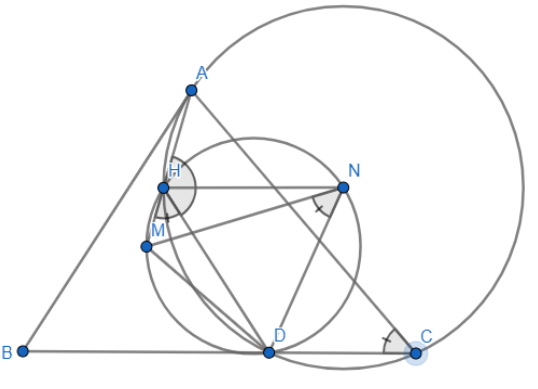
\includegraphics[width=10cm]{proof2.png}

\pagebreak\section{Proof 3 (Quite Easily Done)}

Let $f(x)=x^2-12x+36.$ In terms of $k$, for $k\geq 2,$ find the sum of all real $n$ such that $f^{k-1}(n)=f^k(n).$

\subsection{Solution}

Remark: Most people did not do the following:

\begin{itemize}
	\Item They did not prove that all the roots are distinct.
	
	\Item They did not prove that all the roots are real.
\end{itemize}

First ask why $k\geq 2.$ Answer: $k=1$ gives a weird answer (13).

Make a root tree. Basically you have like, a ton of functions, and it branches off into two more functions. And the sum of the roots of \textbf{each function} stays the same? So it doubles overall.

Now, formalize. We want $f^{k-1}(x)=f^{k}(x),$ so let $f^{k-1}(x)=c.$ Then we just have $c=c^2-12c+36,$ or $c^2-13c+36=0$. This means that either $c=4$ or $c=9.$ By Vieta's both the solutions for $c=4$ and $c=9$ sum to $12.$

\begin{sol}{}{}
Denote $f(x)$ as $z.$ Then for $f(x)=f^2(x),$ we need $z=f(z),$ or $z=z^2-12z+36.$ Then $z$ must be a root of $z^2-13z+36,$ and the roots of this function are $4$ and $9.$
Then we desire $f(x)=4$ or $f(x)=9,$ implying $f(x)-4=f_1(x)=0$ or $f(x)-9=f_2(x)=0.$ By Vieta's Formulas, the sum of the roots of $f_1(x)$ and $f_2(x)$ are both $12.$
Since there are two functions, the sum of all roots is $12\cdot 2=\boxed{24}.$
All the roots are unique because for any function $x^2-12x+c,$ the roots are obviously unique for unique $c.$

Assume this is true for $k.$ Then we prove it is true for $k+1.$ Notice the roots can be paired into roots of $z^2-12z+c$ for some constant $c,$ and all $c$ are unique, so all the roots are unique.
Let the roots be $r_1,r_2\dots r_n.$
Then $f^{k-1}(r_i)=f^k(r_i)$ for all $1\leq i\leq n.$
Let $r_{i1}$ and $r_{i2}$ be the roots of $f(r_{ij})=r_i$ for $1\leq j\leq 2.$
Then all the roots are unique as all prior roots were unique.
By Vieta's Formulas, all of our $2^k$ pairs of roots sum to $12,$ so the total sum is $6\cdot 2^{k+1},$ as desired.

Finally, we have to make sure that all roots are real. Fortunately, we can bound to show all roots are less than or equal to $9,$ showing that they are bounded.
The roots of $f(x)=(x-6)^2=r_i$ are $6\pm \sqrt{r_i}.$ For $x$ to become negative, we need $r_i>36.$ But if for all $r_i$ for any $k,$ $r_i\leq 9,$ then $6+\sqrt{r_i}\leq 9,$ so no roots exceed $9,$ implying none exceed $36.$ We can take the obvious case $k=1$ which has roots $4,9,$ which shows that no roots start out greater than $9.$
\end{sol}

\pagebreak\section{Proof 4}

Consider scalene $\triangle ABC$ with incenter $I.$ Let the $A$ excircle of $\triangle ABC$ intersect the circumcircle of $\triangle ABC$ at $X,Y.$ Let $XY$ intersect $BC$ at $Z.$ Then choose $M,N$ on the $A$ excircle of $\triangle ABC$ such that $ZM,ZN$ are tangent to the $A$ excircle of $\triangle ABC.$ Prove $I,M,N$ are collinear.

\subsection{Interesting thing}

Define $Z_1,Z_2$ in a similar way, then $Z,Z_1,Z_2$ are collinear.

\subsection{Solution}

\begin{itemize}
	\Item Notice we want to prove $I$ lies on $MN,$ aka the polar of $Z.$
	
	\Item La Hire - prove that $Z$ lies on the polar of $I.$
	
	\Item Let the tangents from $I$ to the $A$ excircle be $P,Q$
	
	\Item Notice that $\angle IPI_A=\angle IBI_A=90$ where $I_A$ is the center of the $A$ excircle.
	
	\Item Very obvious from there - draw in $(IBCPQ)$ and use radical axes on $(ABC),(IBCPQ),A$ excircle.
	
	\Item $Z$ lies on $XY$ as desired, La Hire's finishes.
\end{itemize}
    
    \begin{asy}
    size(8cm); 
draw(circle((-4.641800476947178,-3.251291732990515), 2.9355534652731383)); 
draw(circle((-4.651998154130134,-0.9364190124596216), 2.3148951822659347)); 
draw(circle((-4.207275465539313,-6.154507564088528), 4.766411642860937)); 
draw((-5.32,1.28)--(-1.0094263868223374,-2.6200427928750276)); 
draw((-5.32,1.28)--(-8.29981951332241,-3.711197684815037)); 
draw((-6.92,-1.4)--(1.6701428514128647,-1.3621579610069916)); 
draw((-6.6687401853830774,-2.0728569932820617)--(1.6701428514128647,-1.3621579610069916)); 
draw((-5.076325488355045,-0.3480759018925032)--(0.4572846482121191,-7.134588629306881)); 
draw((0.4572846482121191,-7.134588629306881)--(1.6701428514128647,-1.3621579610069916)); 
 /* dots and labels */
dot((-5.32,1.28)); 
label("$A$", (-5.32,1.28), N); 
dot((-6.92,-1.4)); 
label("$B$", (-6.81,-1.11), W); 
dot((-2.38,-1.38)); 
label("$C$", (-2.25,-1.08), E); 
dot((-5.076325488355045,-0.3480759018925032)); 
label("$I$", (-5.07,-0.35),N); 
dot((-6.6687401853830774,-2.0728569932820617)); 
label("$X$", (-6.54,-1.77),0.7S+W); 
dot((-2.472028933738629,-1.7151833561629573)); 
label("$Y$", (-2.47,-1.71),SW); 
dot((1.6701428514128647,-1.3621579610069916)); 
label("$Z$", (1.67,-1.36),NE); 
dot((-4.228272669917007,-1.3881421703520571)); 
label("$M$", (-4.23,-1.39),NE); 
dot((0.4572846482121191,-7.134588629306881)); 
label("$N$", (0.46,-7.13),SW); 
dot((-7.5323969156179205,-2.7395043003379005)); 
label("$P$", (-7.41,-2.43),SE); 
dot((-2.0277141291499343,-1.9156171042963854)); 
label("$Q$", (-2.02,-1.92), SW); 
    \end{asy}

\pagebreak

\begin{sol}{}{}
We want to prove that $I$ lies on the polar of $Z$ with respect to the $A$ excircle. By La Hire's, this is identical to proving that $Z$ lies on the polar of $I.$
    
    Let the tangents from $I$ to the $A$ excircle intersect the $A$ excircle at $P,Q.$ Then we claim that $I,B,C,P,Q$ are concyclic. This is because $\angle IBI_A=\angle ICI_A=\angle IPI_A\angle IQI_A=90^{\circ}.$
    
    Then by the Radical Center Theorem, $Z$ lies on $PQ,$ as desired.
\end{sol}

\pagebreak

 \part{Quiz 1 Discussion}
 
 \setcounter{section}{0}
 \section{Comments}
 
\begin{itemize}

	\Item \textbf{TOO SHORT!} (time limit)

	\Item Problem 1 is the same as Diagnostic 3

	\Item Huh, all happened to be PUMaC 2017, kind of funny

\end{itemize}
\pagebreak


\section{Question 2 (PUMaC Algebra/A 2017/4)}

Let $a_1,a_2,\dots$ be a sequence of positive real numbers such that $a_n=11a_{n-1}-n$ for all $n>1.$ The smallest possible value of $a_1$ can be written as $\frac{p}{q},$ where $p$ and $q$ are relatively prime positive integers. Find $p+q.$

\subsection{Solution}

Like, just find stuff in terms of $a_1.$ Let $a_1=a.$

Then the sequence is

\[a_1,11a_1-1,11^2a_1-11 \cdot 1-2,11^3a_1-1\cdot 11^2-2\cdot 11-3\]

The $11^n$ in front of $a_1$ seems annoying. So kill it! Notice the terms become

\[a_1,a_1-\frac{1}{11},a_1-\frac{1}{11}-\frac{2}{11^2},\cdots\]

So the ``last term'' is $a_1-(\frac{1}{11}+\frac{2}{11^2}+\frac{3}{11^3}+\cdots).$ So just find $\frac{1}{11}+\frac{2}{11^2}+\cdots,$ which is $\frac{21}{100}.$

Answer is $121.$

\pagebreak\section{Question 3 (PUMaC Combo/A 2017/4)}

The four faces of a tetrahedral die are labelled $0, 1, 2,$ and $3,$ and the die has the property that, when it is rolled, the die promptly vanishes, and a number of copies of itself appear equal to the number on the face the die landed on. For example, if it lands on the face labelled $0,$ it disappears. If it lands on the face labelled $1,$ nothing happens. If it lands on the face labelled $2$ or $3,$ there will then be $2$ or $3$ copies of the die, respectively (including the original). Suppose the die and all its copies are continually rolled, and let $p$ be the probability that they will all eventually disappear. Find $\left\lfloor \frac{10}{p} \right\rfloor$.

\subsection{Solution}

States.

If there are $2$ die, the probability of them both disappearing is $p^2,$ etc. This is the main and only observation.

Just do algebra now.

\[p=\frac{1}{4}(1+p+p^2+p^3)\]
Note that $p=\sqrt{2}-1.$

So the answer is $\lfloor\frac{10}{\sqrt{2}-1}\rfloor=\lfloor10\sqrt{2}+10\rfloor=24.$

\pagebreak\section{Question 4 (PUMaC Algebra/A 2017/7)}

The sum
    \[\sum_{k=0}^{\infty} \frac{2^{k}}{5^{2^{k}}+1}\]
    can be written in the form $\frac{p}{q}$ where $p$ and $q$ are relatively prime positive integers. Find $p+q$.

\subsection{Solution}

Notice this is equal to

% I am scared. 
\[\sum\limits_{n=1}^{\infty}\frac{2^k(5^{2^k}-1)}{(5^{2^{k+1}}-1)}=\]
\[\sum\limits_{n=1}^{\infty}\frac{2^k}{5^{2^k}-1}-\frac{2^{k+1}}{5^{2^{k+1}}-1}=\]
\[\frac{2^0}{5^{2^0}-1}=\frac{1}{4}.\]
\end{document}
